\documentclass[11pt]{article}
\usepackage[a4paper,margin=1in]{geometry}
\usepackage{amsmath,amssymb}
\usepackage{graphicx}
\usepackage{booktabs}
\usepackage{xcolor}
\usepackage[colorlinks=true,linkcolor=blue,citecolor=blue,urlcolor=blue]{hyperref}
\usepackage{caption}
\captionsetup{font=small,labelfont=bf}
\graphicspath{{./}}

\newcommand{\MKK}{M_{\mathrm{KK}}}
\newcommand{\epsK}{\varepsilon_K}
\newcommand{\dmK}{\Delta m_K}
\newcommand{\TeV}{\,\mathrm{TeV}}
\newcommand{\GL}{(G_L^d)}
\newcommand{\GR}{(G_R^d)}

\title{\bf Three CP invariants, not one: what actually has to be aligned to
fix $\epsK$ in warped flavor\\[4pt]
\large A survival-mechanism anatomy of anarchic Randall-Sundrum, with a
numerically demonstrated negative result}
\author{5D-Neutrino-Mixing project, RS-FLAVOR-ALIGNMENT-2026-07}
\date{July 2026}

\begin{document}
\maketitle

\begin{abstract}
\noindent
Anarchic Randall-Sundrum (RS) is pushed to $\MKK\gtrsim 10$--$20\TeV$ almost
entirely by the CP-violating kaon amplitude $\epsK$, generated by the
chirality-enhanced KK-gluon operator $C_4$. The standard responses align the
Yukawas so as to suppress the \emph{magnitude} of the dangerous coupling
(right-handed down $U(3)$, $5$D-MFV, flavor shining). We ask a sharper question:
what is the minimal set of CP structures that a low-$\MKK$ RS point must control,
and does aligning the kaon operator suffice. Working from a forward Monte Carlo
that retains the full complex down-sector couplings, we establish three things.
(i) Anarchic $\epsK$ survival at $\MKK\le3\TeV$ is \emph{magnitude-dominated}:
about $57\%$ of survivors have an accidentally small $|C_4|$ and only about $7\%$
survive by a genuine CP-phase cancellation. This is a consequence of the cut
itself, which weights survivors by a phase-volume factor $P_{\rm pass}(R_K)\sim
1/R_K$. (ii) A ``CP-only'' alignment that makes the down Yukawa real kills the
kaon phase exactly and passes $\epsK$ at $100\%$ \emph{while keeping the coupling
magnitude anarchic}, so $\dmK$ stays large. This is a distinct corner from the
magnitude cures. (iii) That same point is \emph{not} EDM-safe: the neutron-EDM CP
invariant $I_d=\mathrm{Im}\,[F_Q(Y_uY_u^\dagger+Y_dY_d^\dagger)Y_dF_d]_{11}$ stays
$O(1)$, sourced by up-sector CP through $Y_uY_u^\dagger$, independent of the kaon
phase. The kaon operator and the neutron EDM are governed by \emph{different} CP
invariants; aligning one does not align the other. The practical consequence is
that ``sequester CP'' is not one condition but (at least) two, and the
$(\dmK,\,d_n)$ plane separates every candidate mechanism. The genuinely open,
buildable target is a calculable construction that suppresses the kaon operator
\emph{magnitude} (rank-one / $U(2)$ localization) \emph{and} confines CP in the
strong Nelson-Barr sense (real determinant), because neither alone is sufficient.
\end{abstract}

\section{The obstruction, stated precisely}
The RS-GIM mechanism suppresses most quark flavor violation once $\MKK$ is
electroweak-safe, with the single robust exception of $\epsK$~\cite{CFW,Blanke},
and a subdominant $D^0$ concern. In this repo's convention the binding operator is
the color-octet KK-gluon left-right operator,
\begin{equation}
  C_4 = -\,\frac{\GL_{12}\GR_{12}}{\MKK^2},\qquad
  \GL_{12}\sim g_{s*} f_{Q_1}f_{Q_2}\,e^{i\phi_L},\quad
  \GR_{12}\sim g_{s*} f_{d_1}f_{d_2}\,e^{i\phi_R},
\end{equation}
with $\phi_{L,R}$ order-one anarchic phases. Writing $R_K\equiv 2|M_{12}^{LR}|/\dmK$
and $\theta_K\equiv\arg[\GL_{12}\GR_{12}]$,
\begin{equation}
  |\epsK^{\rm NP}| \simeq \frac{\kappa_\epsilon}{2\sqrt2}\,R_K\,|\sin\theta_K|
  \simeq 0.332\,R_K\,|\sin\theta_K|,\qquad
  \dmK^{\rm NP}\propto R_K\cos\theta_K .
\end{equation}
So $\epsK$ measures $R_K\sin\theta_K$ and $\dmK$ measures $R_K\cos\theta_K$: the same
magnitude $R_K$, projected on the imaginary and real axes. A low-$\MKK$ survivor can
therefore be built two ways, by small $R_K$ (small magnitude) or by small
$\sin\theta_K$ (aligned phase). These are physically different and, as we show, they
predict different things.

\section{F1: anarchic survival is magnitude-dominated}
From a $9.9\times10^5$-draw anarchic ensemble (masses and CKM fit per draw), the
$\epsK$ survivors at $\MKK\le3\TeV$ split (Fig.~\ref{fig:plane}) into
\emph{magnitude-suppressed} ($\sim$57\%, small $|C_4|$, which also makes $\dmK$
small) and \emph{phase-aligned} ($\sim$7\%, $|C_4|$ anarchic, $\sin\theta_K\to0$,
$\dmK$ saturating). The dominance of the magnitude mode is not an independent fact:
the $\epsK$ cut weights the pre-cut population by the phase volume
\begin{equation}
  P_{\rm pass}(R_K)=\frac{2}{\pi}\arcsin\!\Big(\frac{\epsilon_{\max}}{0.332\,R_K}\Big)
  \xrightarrow{\,R_K\gg\,} \frac{2\,\epsilon_{\max}}{\pi\,0.332}\,\frac{1}{R_K},
\end{equation}
so large-magnitude points are penalized as $1/R_K$ and survivors tilt to small
$|C_4|$. The measured correlation $\mathrm{corr}(\log\epsK,\log\dmK)=+0.82$ is the
signature: a pure phase-cancellation picture would give an anticorrelation. The
practical lesson is that ``anarchy survives by fine-tuning the $\epsK$ phase'' is the
\emph{minority} path; most survivors simply draw a small coupling.

\begin{figure}[t]
  \centering
  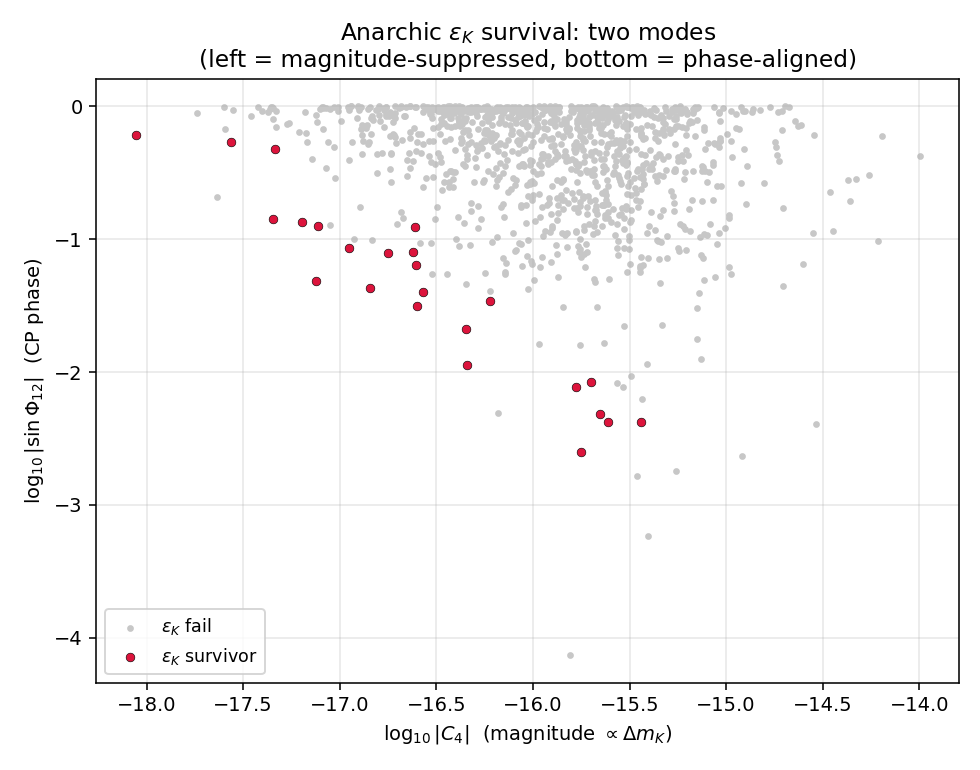
\includegraphics[width=0.62\textwidth]{fig_F1_survival_plane.png}
  \caption{Anarchic $\epsK$ survival in the (magnitude, phase) plane at
  $\MKK=3\TeV$. Survivors (red) populate two disjoint regions: the left edge (small
  $|C_4|$, magnitude-suppressed) and the bottom edge (small $|\sin\Phi_{12}|$,
  phase-aligned). The bulk is the magnitude edge.}
  \label{fig:plane}
\end{figure}

\section{The three CP invariants}
The point of this note is that a low-$\MKK$ RS quark sector must control more than one
CP structure, and they are independent:
\begin{itemize}\itemsep2pt
\item $\theta_K=\arg[\GL_{12}\GR_{12}]$ sets $\epsK$ (kaon $1$-$2$, left-right).
\item $I_d=\mathrm{Im}\,[F_Q(Y_uY_u^\dagger+Y_dY_d^\dagger)Y_dF_d]_{11}/(\text{mass})$
  sets the neutron EDM. The tree KK-gluon EDM vanishes (the diagonal couplings are
  real); the leading RS contribution is the one-loop Higgs/KK-fermion dipole with the
  \emph{misaligned} spurion $Y_uY_u^\dagger+Y_dY_d^\dagger$~\cite{APS}.
\item $\theta_D=\arg[(G_L^u)_{12}(G_R^u)_{12}]$ sets $D^0$ CP violation (up $1$-$2$).
\end{itemize}
The crucial feature is that $I_d$ feeds on $Y_uY_u^\dagger$: up-sector CP enters the
down-quark EDM directly, with no reference to the kaon phase $\theta_K$.

\section{F2/F3: CP-only alignment fixes $\epsK$ but not the EDM}
Consider the cleanest CP-only alignment: a real anarchic down Yukawa, with CP carried
by the up sector (a Nelson-Barr-like routing that keeps a realistic Jarlskog $J$). By
construction the down $M_d$ is real, so $\theta_K=0$ and $\epsK$ vanishes at tree
level, while $|C_4|$ is untouched. The forward Monte Carlo confirms this and adds the
decisive point (Table~\ref{tab:disc}, Fig.~\ref{fig:disc}):
\begin{table}[h]
  \centering
  \caption{Mechanism comparison at $\MKK=3\TeV$ (PDG$+J$-passing points).
  $|C_4|$ is the $\dmK$ proxy; $|I_d|$ is the neutron-EDM CP invariant.}
  \label{tab:disc}
  \begin{tabular}{lcccc}
    \toprule
    Lane & $\epsK$ pass & $|\sin\theta_K|$ & $\log_{10}|C_4|$ & $|I_d|$ (EDM) \\
    \midrule
    flat anarchy                 & $2\%$   & $0.54$      & $-15.9$ & $2.9$ \\
    magnitude align ($U(3)_{d_R}$) & high  & --           & suppressed & suppressed \\
    \textbf{CP-only (real $Y_d$)} & $\mathbf{100\%}$ & $\mathbf{10^{-16}}$ & $\mathbf{-15.9}$ & $\mathbf{4.1}$ \\
    \midrule
    sanity: fully real $Y_{u,d}$ & --      & $10^{-16}$   & --      & $0.0$ \\
    \bottomrule
  \end{tabular}
\end{table}

A real down sector passes $\epsK$ at $100\%$ with the coupling magnitude at its
anarchic value (so $\dmK$ stays large), yet the EDM invariant is $|I_d|\simeq4$,
\emph{larger} than flat anarchy. Turning up-sector CP off (fully real Yukawas) sends
$I_d\to0$ exactly, confirming both the estimator and the mechanism: the residual EDM
is up-sector CP leaking through $Y_uY_u^\dagger$. Aligning the kaon operator does
nothing to it. This is the central result: \textbf{CP-only alignment of the kaon
operator does not yield an EDM-safe theory}. An EDM cure requires controlling the
up-sector CP as well, which is precisely what genuine Nelson-Barr (a real quark mass
determinant, CP confined to a heavy sector) delivers and a merely real $Y_d$ does not.

\begin{figure}[t]
  \centering
  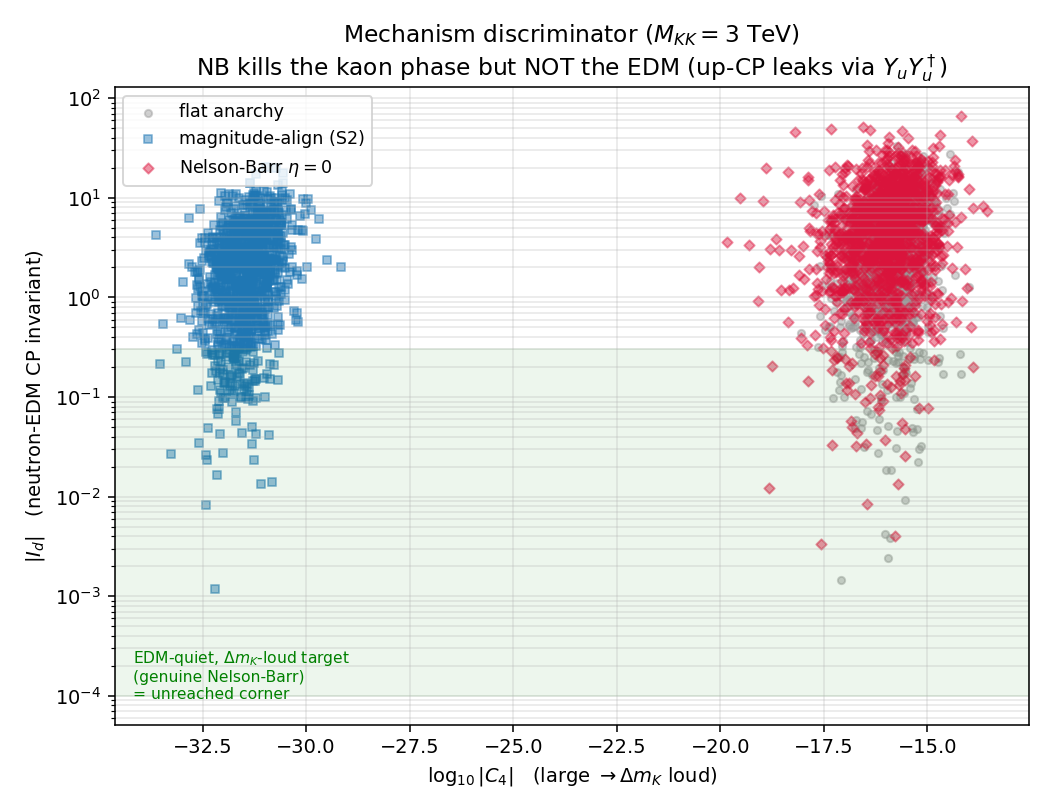
\includegraphics[width=0.66\textwidth]{fig_mechanism_discriminator.png}
  \caption{The $(\dmK,\,d_n)$ discriminator at $\MKK=3\TeV$. Magnitude alignment
  moves left (small $|C_4|$, $\dmK$ quiet); CP-only alignment stays right ($\dmK$
  loud) but high in $|I_d|$ (EDM loud). The green EDM-quiet, $\dmK$-loud corner
  (genuine Nelson-Barr) is not reached by any single-axis anarchic draw.}
  \label{fig:disc}
\end{figure}

\section{What is new, and what is not}
The broad ideas here are not new and we do not claim them. CP-only / minimal-CP
suppression of $\epsK$ with reduced EDMs exists in composite/warped language
(Redi-Weiler~\cite{RediWeiler}); warped Nelson-Barr with CP moved to a heavy sector
exists (Girmohanta et al.~\cite{Girmohanta}); the magnitude cures are FPR
$5$D-MFV~\cite{FPR}, Santiago right-handed-down protection~\cite{Santiago}, and
flavor shining~\cite{Shining}; CP sequestering in warped space is
Cheung-Fitzpatrick-Randall~\cite{CFR}. The defensible, and to our knowledge
unpublished, content is narrower:
\begin{enumerate}\itemsep2pt
\item the survival-mechanism taxonomy of Sec.~2, with the $P_{\rm pass}\sim1/R_K$
  explanation of why anarchic survival is magnitude-dominated;
\item the explicit demonstration that the kaon phase and the neutron-EDM invariant
  are independent, so that a real down sector is $\epsK$-safe with anarchic $\dmK$ yet
  EDM-loud (Sec.~5), i.e.\ CP-only kaon alignment is provably insufficient;
\item the $(\dmK,\,d_n)$ plane as a mechanism discriminator that separates
  magnitude alignment, CP-only alignment, and genuine Nelson-Barr into distinct,
  falsifiable corners.
\end{enumerate}

\section{The worked target}
The synthesis the literature points to, and that our numerics motivate operationally,
is a single calculable construction combining two independent ingredients, because we
have shown neither suffices alone:
\begin{itemize}\itemsep2pt
\item \textbf{Magnitude:} a sequentially generated, low-rank Yukawa ensemble under an
  accidental light-family $U(2)$ symmetry (rather than i.i.d.\ anarchy), so that the
  KK-gluon $1$-$2$ coupling is structurally, not accidentally, small. This is the
  ``wrong ensemble'' correction: natural Yukawas are rank-one towers, not flat random
  matrices, and the resulting $\epsK$ floor is set by symmetry-breaking leakage rather
  than phase luck.
\item \textbf{CP:} genuine Nelson-Barr confinement of CP (real mass determinant), so
  that both $\theta_K$ \emph{and} $I_d$ are spurion-suppressed, not just the kaon
  phase. A real $Y_d$ alone is demonstrably not enough.
\end{itemize}
Each ingredient exists separately; no calculable $5$D construction combines them with
a controlled radiative-stability proof. The decisive metric for such a build is the
scale $M_{50}$ at which at least half of the points pass \emph{all} constraints
(masses, CKM, $\epsK$, $\dmK$, $B_{d,s}$, $D^0$, and the EDM invariant), compared
across flat anarchy, magnitude-only, CP-only, and the combined construction. Our
results predict that only the combined construction reaches the few-TeV regime with
$\dmK$ retained and $I_d$ suppressed.

\section{Bottom line}
The RS $\epsK$ problem has been read as a problem of one delicate phase in the
off-diagonal down couplings. It is really a problem of \emph{three} independent CP
structures, of which the kaon phase is only one. Aligning the kaon operator, by
magnitude or by phase, leaves the neutron EDM untouched, because the EDM samples a
flavor-diagonal invariant fed by the up sector. A low-$\MKK$ warped flavor model is
therefore not ``anarchy plus one alignment relation''; it must suppress the kaon
operator magnitude with a low-rank, $U(2)$-symmetric ensemble and confine CP in the
Nelson-Barr sense, together, in one calculable construction. That combined target,
and the $(\dmK,\,d_n)$ discriminator that certifies it, is the concrete next step.

\begin{thebibliography}{9}
\small
\bibitem{CFW} C.~Cs\'aki, A.~Falkowski, A.~Weiler, arXiv:0804.1954.
\bibitem{Blanke} M.~Blanke et al., arXiv:0809.1073.
\bibitem{APS} K.~Agashe, G.~Perez, A.~Soni, hep-ph/0408134 (RS CP problem / neutron EDM).
\bibitem{FPR} A.~L.~Fitzpatrick, G.~Perez, L.~Randall, arXiv:0710.1869 ($5$D-MFV).
\bibitem{Santiago} J.~Santiago, arXiv:0806.1230 (minimal flavor protection).
\bibitem{Shining} C.~Cs\'aki, G.~Perez, Z.~Surujon, A.~Weiler, arXiv:0907.0474 (flavor shining).
\bibitem{CFR} C.~Cheung, A.~L.~Fitzpatrick, L.~Randall, arXiv:0711.4421 (CP sequestering).
\bibitem{RediWeiler} M.~Redi, A.~Weiler, arXiv:1106.6357 (minimal CP violation).
\bibitem{Girmohanta} S.~Girmohanta, S.~J.~Lee, Y.~Nakai, M.~Suzuki, arXiv:2203.09002 (warped Nelson-Barr).
\bibitem{GT} A.~Greljo, A.~E.~Thomsen (rank-one sequential Yukawas); Barbieri et al.\ $U(2)$ flavor.
\end{thebibliography}
\end{document}
